\documentclass[a4paper]{article}

\usepackage[english]{babel}
\usepackage[utf8x]{inputenc}
\usepackage{amsmath}
\usepackage{amsfonts}
\usepackage{graphicx}
\usepackage[colorinlistoftodos]{todonotes}

\title{CS 5785 - Applied Machine Learning - Lec.\ 4}
\author{Prof.\ Nathan Kallus, Cornell Tech\\Scribe: Jake Bass, Steffen Baumgarten, Zimeng Zhu}
\date{September 4, 2018}

\begin{document}
\maketitle
\section{Conditional Expectation is the Best Regression Model}
As we can see, kNN and OLS(ordinary least squares) are some regression model, but which one is the best regression model? We should consider one that minimize $R(f)=E[\ell(Y,f(x))]$ ,in which X,Y are random variables representing new random examples.\newline
We can start by doing a preliminary warm up:Let's consider given a random variable Y, which $c\in R$ minimize $E[(Y-c)^2]$?\newline
$$\frac{\partial}{\partial c}E[(Y-c)^2]=E[\frac{\partial}{\partial c}(Y-c)^2]$$
$$=E[2(c-Y)]$$
$$=2c-2EY$$
So that we need to solve $2c-2EY=0$,which leads to$c*=EY$.
In a nutshell, the mean(average) is the single constant number that's simultaneously closest to all values of a random Y in average squared distance.\newline
Now we can consider minimizing the risk based on our preliminary method, which is:\newline
$$R(f)=E[(Y-f(x))^2]=E[E[((Y-f(x))^2|x]]$$\newline
And what should $f(x)$ be? We can tell according to the warm up conclusion that$f*(x)=E[Y|X=x]$ is the optimal prediction.\newline
OLS regression estimating the conditional mean, and conditional expectations, probabilities and modes are the primary targets of Supervised Learning.


\section{Linear Model for Classification}
\subsection{Log Odds}
Focus on binary classifcation $G=\{0,1\}$. \newline
Recall, Bayes classifier declares $\hat{Y}=1$ when $Pr(Y=1|X=x) > Pr(Y=0|X=x)$. \newline
Look at the odds ratio: \newline
$$OR = \frac{\text{Pr}(Y=1|X=x)}{\text{Pr}(Y=0|X=x)} \in [0, \infty]$$ \newline
Then, to transform it to a number in $(-\infty, \infty)$: \newline
Log odds: 
$$log(\frac{\text{Pr}(Y=1|X=x)}{\text{Pr}(Y=0|X=x)})$$
$$ = log(\frac{\text{Pr}(Y=1|X=x)}{1 - \text{Pr}(Y=1|X=x)})$$
$$ = logit(\text{Pr}(Y=1|X=x)) $$
where $logit(P) = log(\frac{P}{1-P}) = log(\frac{1}{\frac{1}{P} - 1}) = log(P) - log(1-p)$. \newline
So, the domain of the logit is $P \in [0,1]$, and the co-domain is $[-\infty, \infty]$. \newline
This means that $logit(\text{Pr}(Y=1|X=x))$ is a score for declaring $\hat{Y}=1$ that is symmetric. When it is positive, we can declare $\hat{Y}=1$; when it is negative, we can declare $\hat{Y}=0$.

\begin{figure}[h!]
\centering
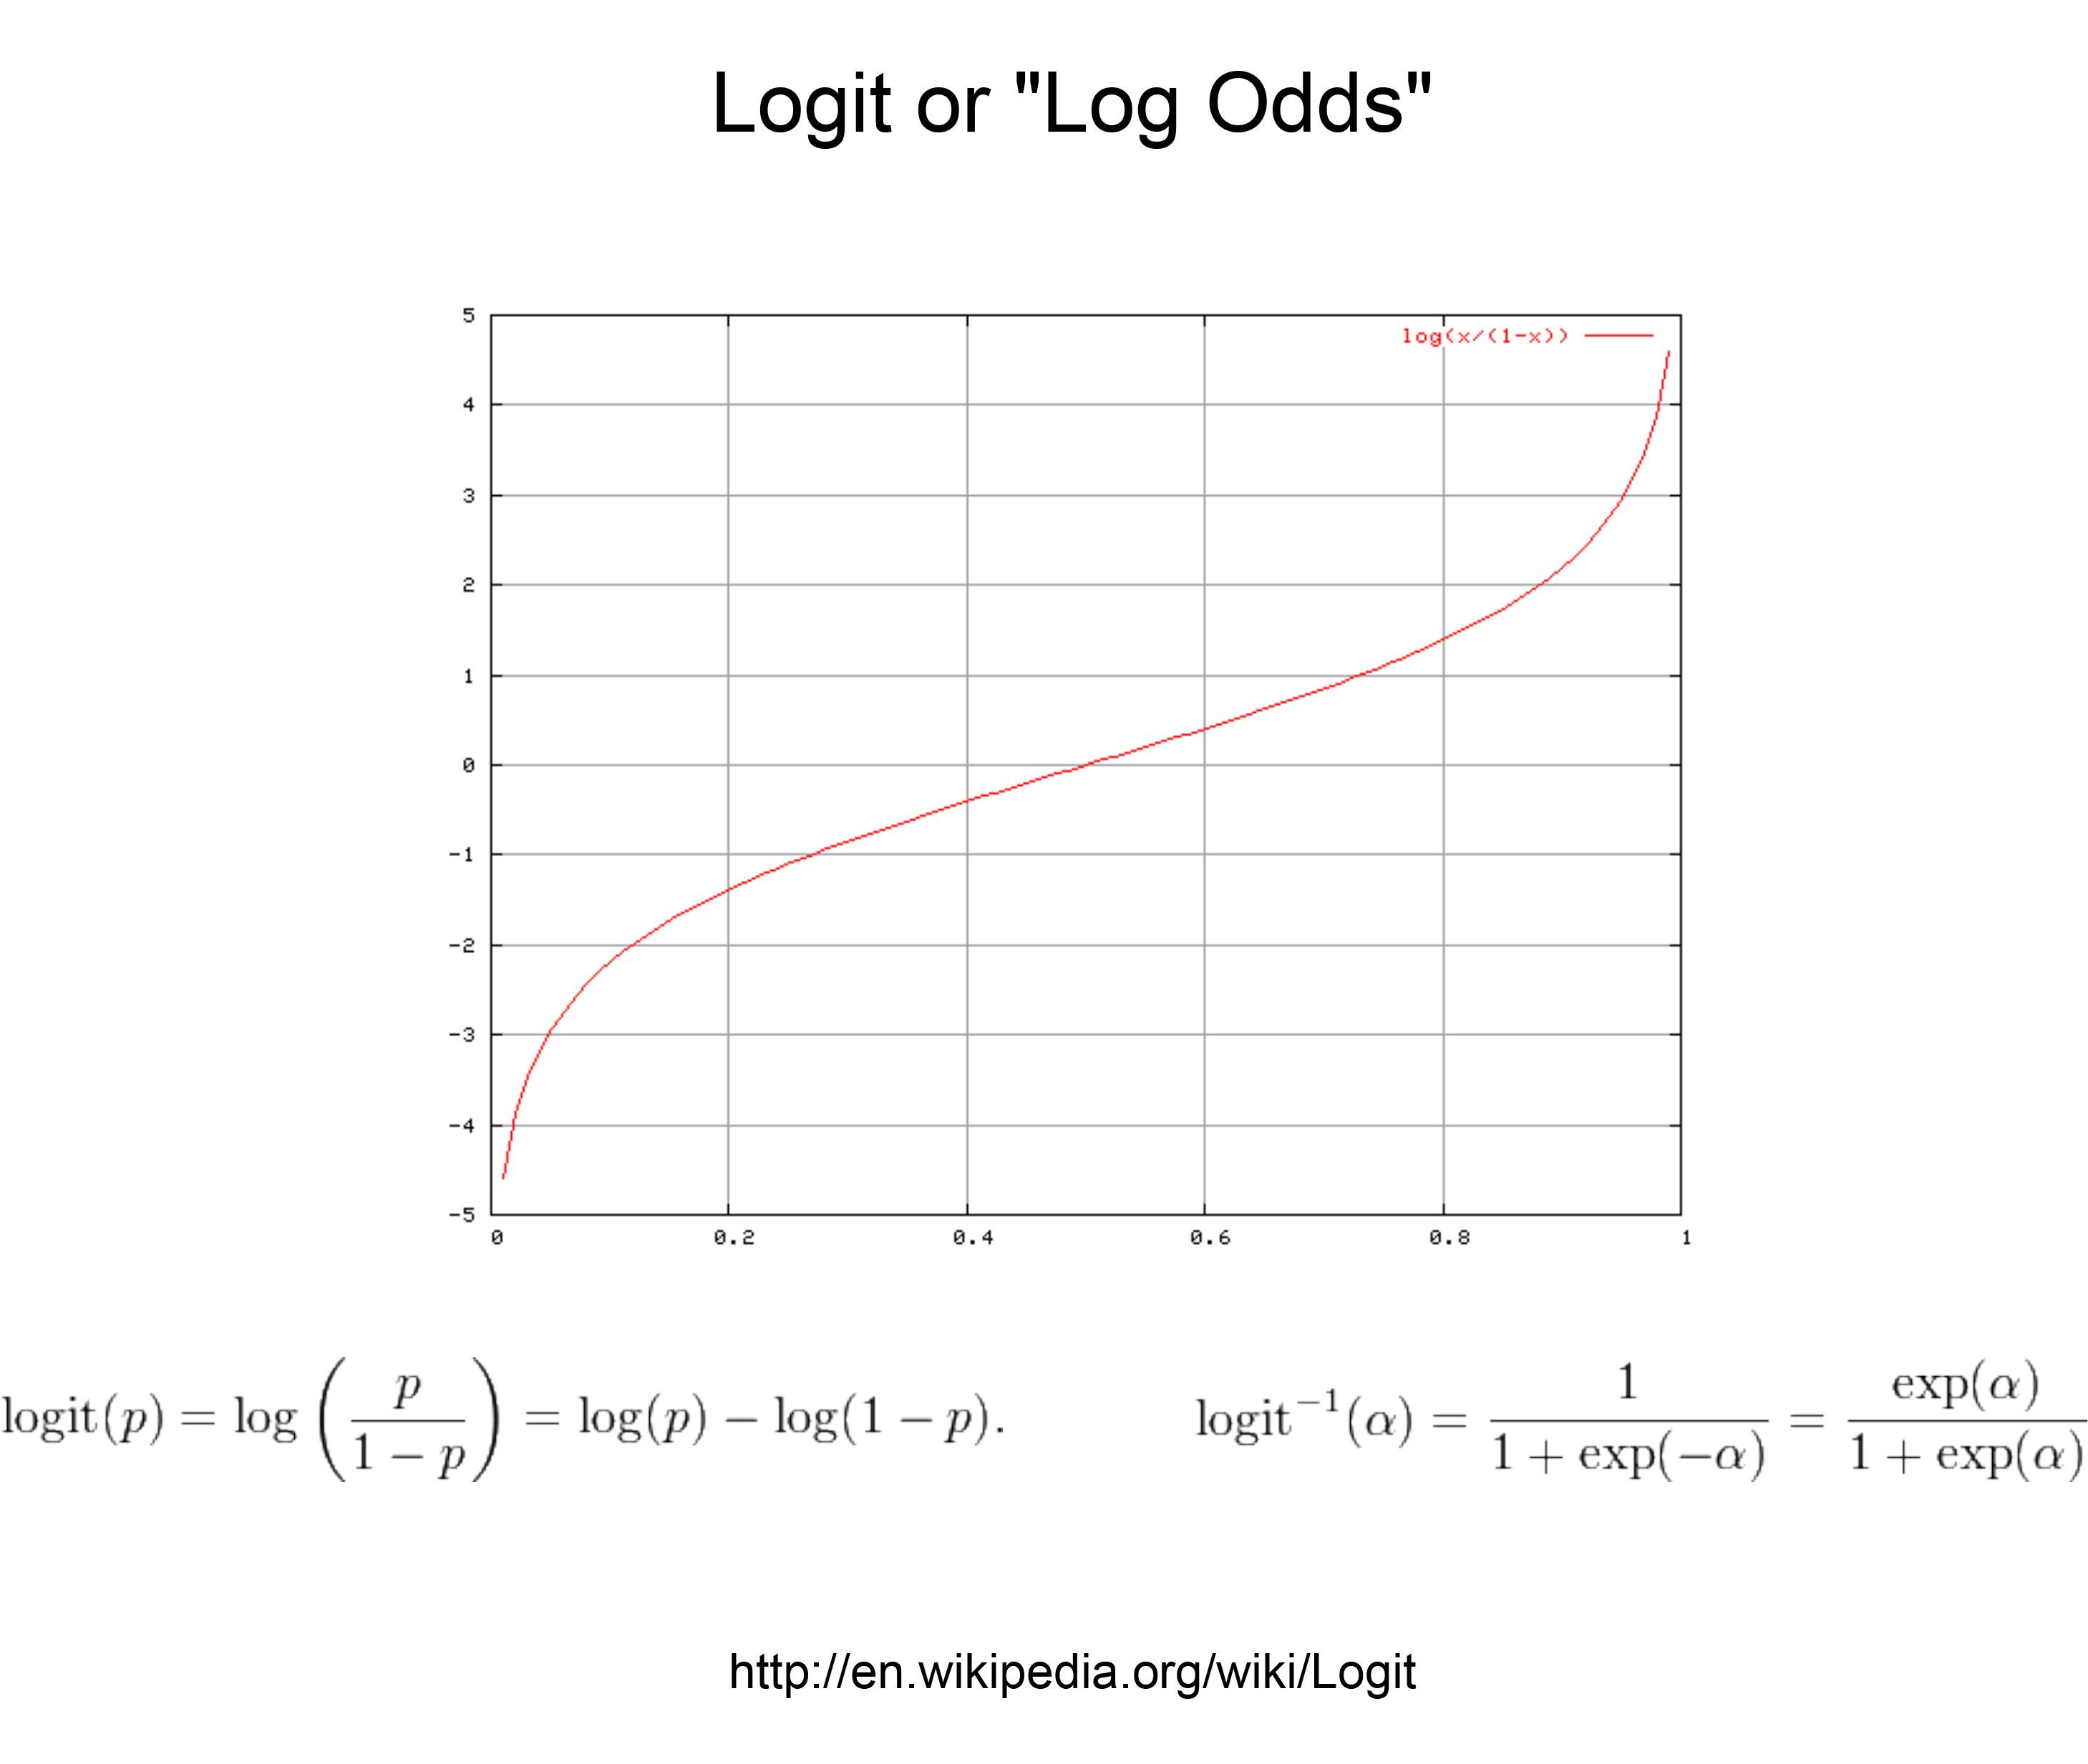
\includegraphics[width=0.75\textwidth]{logit.png}
\end{figure}

\subsection{Logistic Regression}
Posit $Logit(P(Y=1 | X=x)) = \beta^\top X => P(Y=1 | X = x) = \sigma(\beta^\top X)$ \newline
where $\sigma$ is the logistic sigmoid: $\sigma(z) = logit^{-1}(z) = \frac{1}{1 + exp(-z)} = \frac{exp(z)}{1 + exp(z)}$ \newline
$\sigma$ gives a way to transform a score $\beta^\top X$ into a probability. 
You can see:
$$ \sigma(0) = \frac{1}{2}$$
$$ \sigma(\infty) = 1 $$
$$ \sigma(- \infty) = 0 $$
$$ \sigma(- z) = 1 - \sigma(z) $$
$$ \frac{\partial \sigma}{\partial z} = \frac{-1}{(1 + e^{-z})^2} \cdot (-e^{-z}) = \frac{e^-z}{(1 + e^{-z})^2} $$
$$= \frac{1}{1+e^{-z}} \cdot \frac{e^{-z}}{1+e^{-z}}= \frac{1}{1 + e^{-z}} \cdot (1 - \frac{1}{1 + e^{-z}})= \sigma(z) \cdot (1 - \sigma(z)) $$

\begin{figure}[h!]
\centering
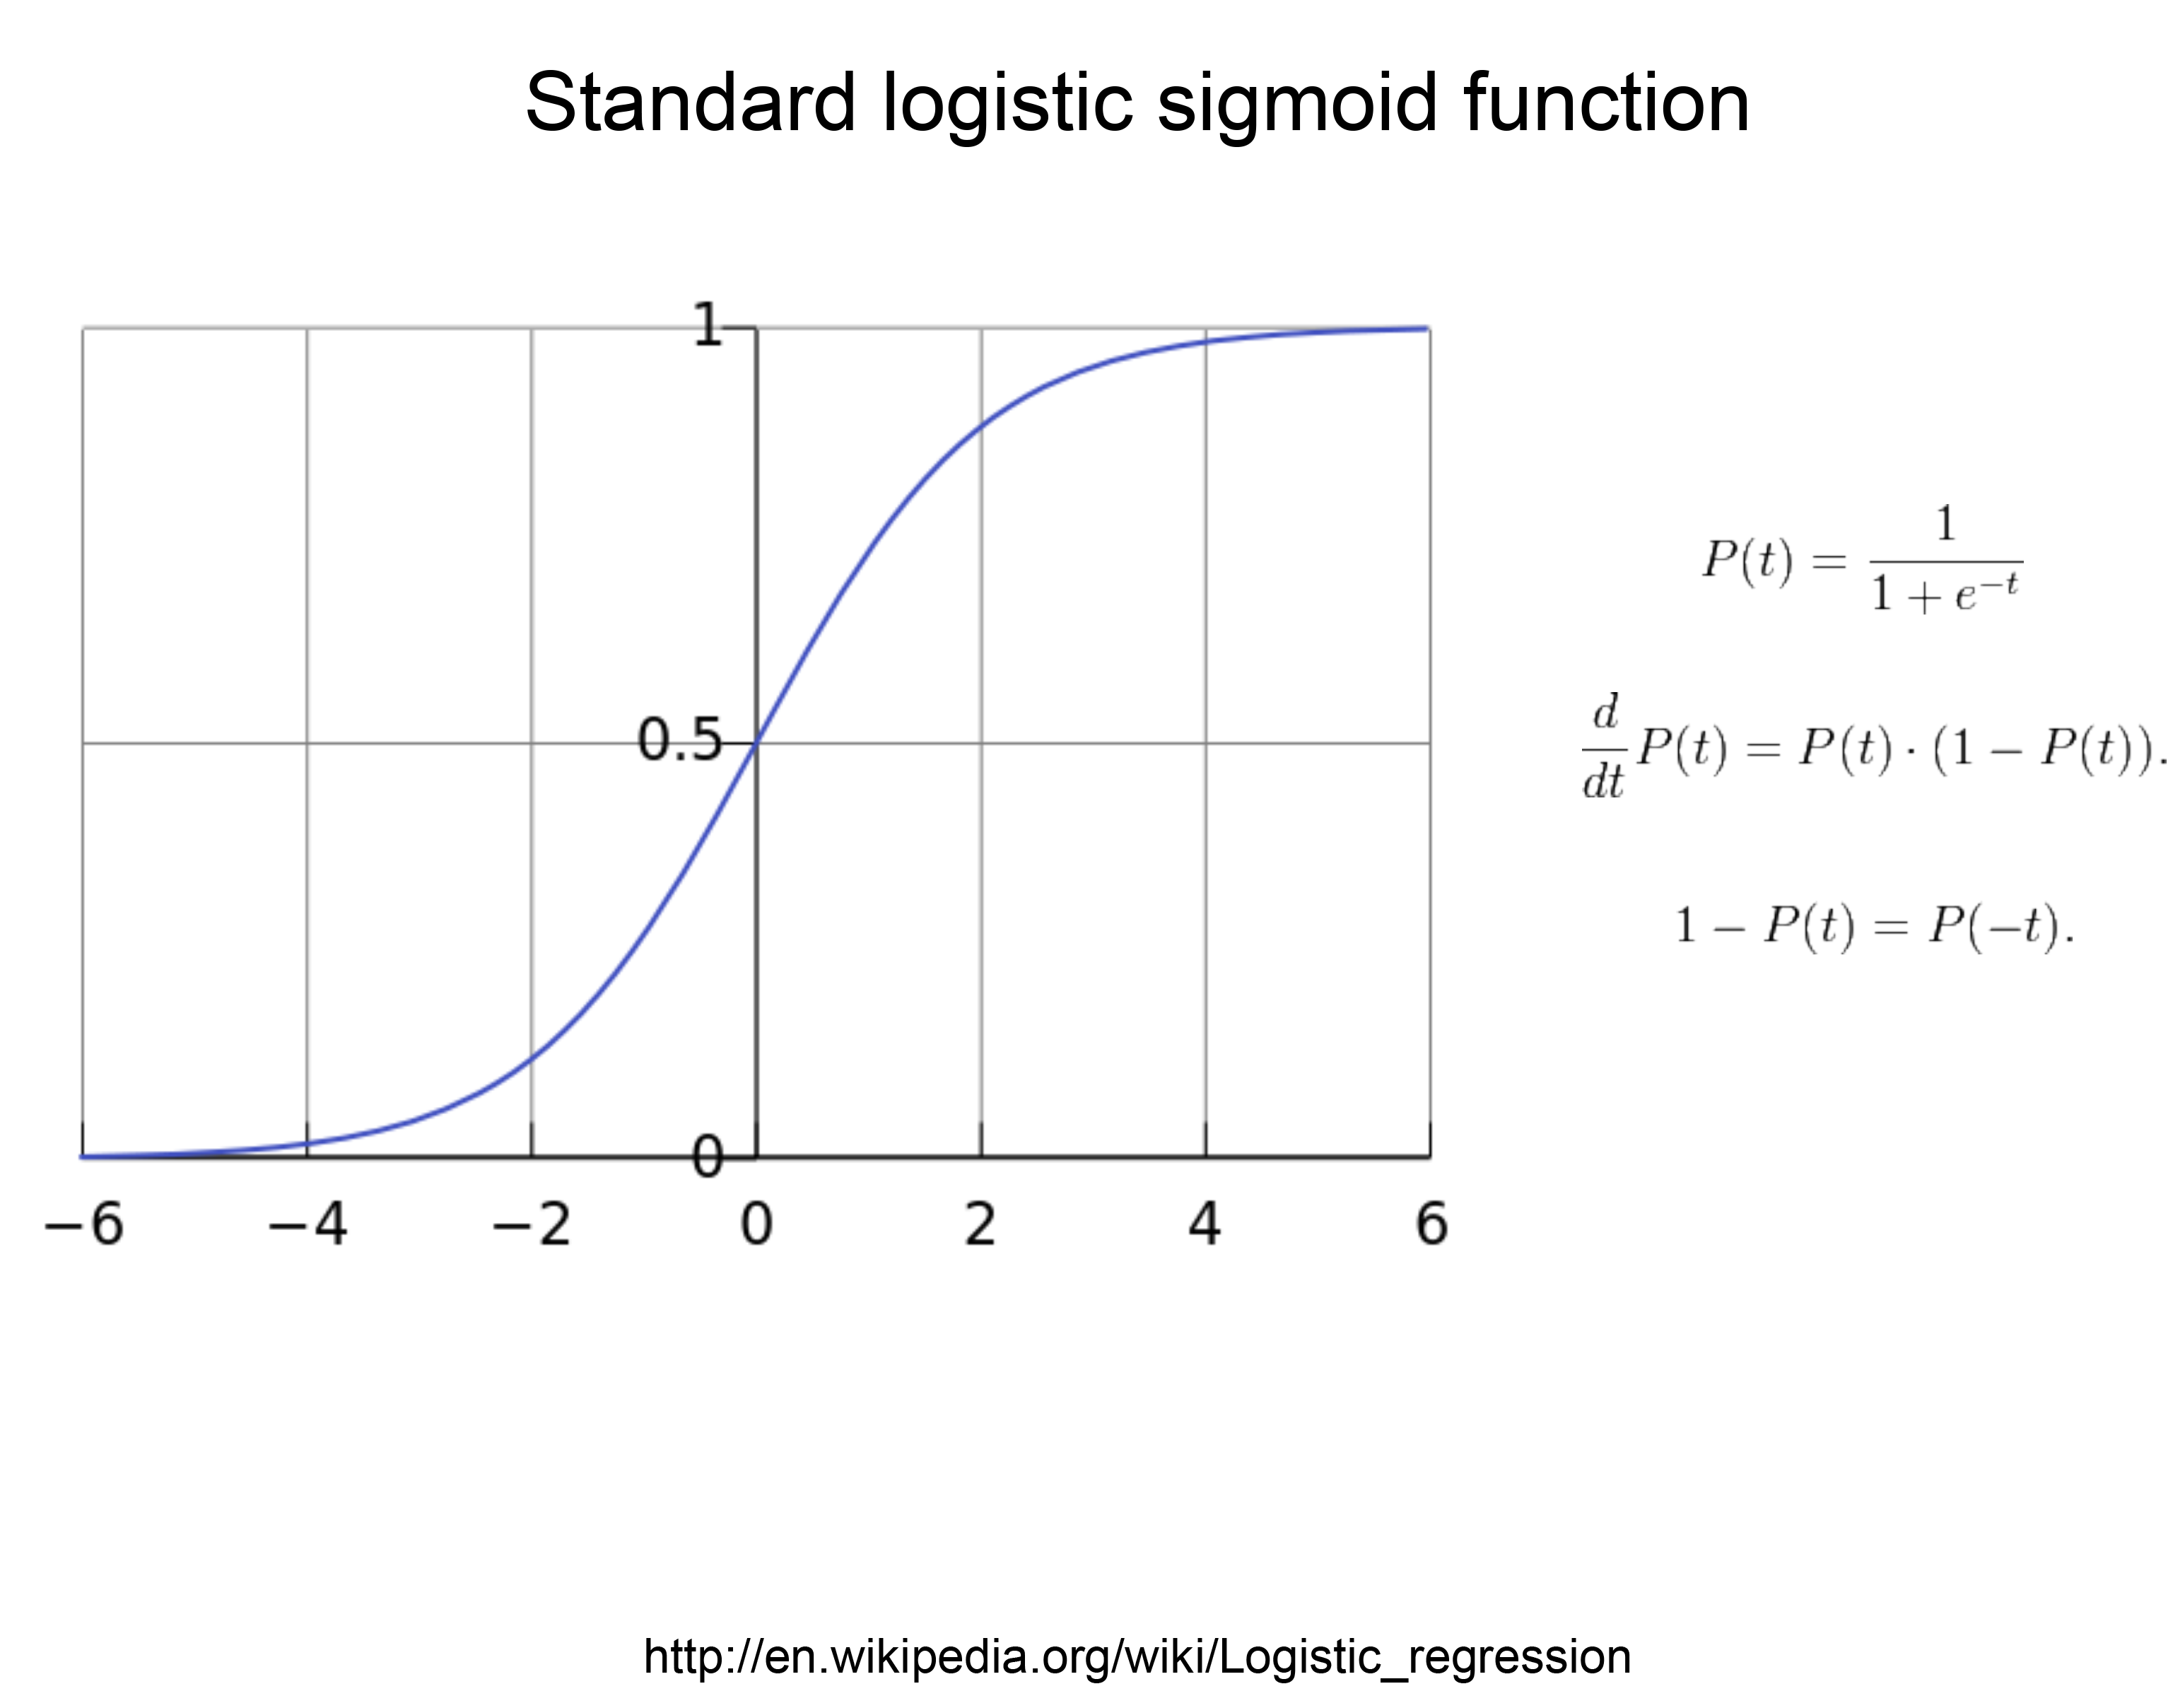
\includegraphics[width=0.75\textwidth]{sigmoid.png}
\end{figure}

\subsection{Fitting Logistic Regression: Maximum Likelihood}
Logistic regression provides a \underline{generative model} for the data. That is, it provides a model that specifies how the data was generated given x. Logistic regression specifies $P(Y=1 | X =x) = \sigma(\beta^\top X)$. That is, draw an $X$, get a $\sigma(\beta^\top X)$; flip a biased coin with that probability of a head and label the example heads or tails accordingly. Alternatively, it can be thought of a such: generate $\mathcal{U} \sim Uniform[0,1]$ and label 1  if $\mathcal{U} < \sigma(\beta^\top X)$, and otherwise label 0. \newline

Assuming that the data is independent, for every $\beta$ there is a particular likelihood for observing the data we did:\newline
$$Lik(\beta)=P(X_1,Y_1,......,X_n,Y_n;\beta)$$
$$=\prod_{i=1}^N P(X_i,Y_i;\beta)$$
$$ =\prod_{i=1}^N P(Y_i|X_i;\beta)P(X_i)$$
$$ =\prod_{i=1}^N P(X_i)(
\begin{cases} 
      \sigma(\beta^\top X_i) & if  Y_i=1 \\
      1-\sigma(\beta^\top X_i) & if  Y_i=0 \\
\end{cases})
$$
Max likelihood's principle is choose parameters that maximize the likelihood of observing the data we observed.\newline
Since log is monotonic increasing, so we can conclude that:\newline
$$argmax Lik(\beta)=argmax log(Lik(\beta))=argmin[-log(Lik(\beta))]$$\newline
And:
$$-log(Lik(\beta))=\sum_{i=1}^N (-logP(X_i)-(\begin{cases} 
      \sigma(\beta^\top X_i) & if  Y_i=1 \\
      1-\sigma(\beta^\top X_i) & if  Y_i=0 \\
\end{cases}))$$
$$=-\sum_{i=1}^NlogP(X_i)+\sum_{i=1}^N(Y_i(-log\sigma(\beta^\top X_i)+
(1-Y_i)(-log(1-\sigma(\beta^\top X_i))))$$
In this part, we can define negative log likelihood function as:\newline
$$\mathcal{L}(\beta)=\sum_{i=1}^N(Y_i(-log\sigma(\beta^\top X_i)+
(1-Y_i)(-log(1-\sigma(\beta^\top X_i))))$$\newline
So basically $argmax Lik(\beta)$ is equal to $argmin \mathcal{L}(\beta)$now\newline
Since:\newline
$$log(\sigma(\beta^\top X_i))=log(\frac{e^{\beta^\top X_i})}{1+e^{\beta^\top X_i}}$$
$$=\beta^\top X_i-log(1+e^{\beta^\top X_i})$$\newline
And:\newline
$$log(1-\sigma(\beta^\top X_i))=log(\sigma(-\beta^\top X_i))$$
$$=log(\frac{1}{1+e^{\beta^\top X_i}}$$
$$=-log(1+e^{\beta^\top X_i})$$
So finally we get:\newline
$$\mathcal{L}(\beta)=\sum_{i=1}^N(Y_i log(1+e^{\beta^\top X_i})-Y_i\beta^\top X_i+(1-Y_i)log((1+e^{\beta^\top X_i}))$$
$$=\sum_{i=1}^N(log(1+e^{\beta^\top X_i})-Y_i\beta^\top X_i)$$

\end{document}
